\section{Simulation Analysis}
\label{sec:simulation}

\subsection{Operating Point Analysis}


The Table~\ref{tab:op} shows the simulated operating point results for the circuit described in Figure~\ref{fig:circuito}.

\begin{figure}[h] \centering
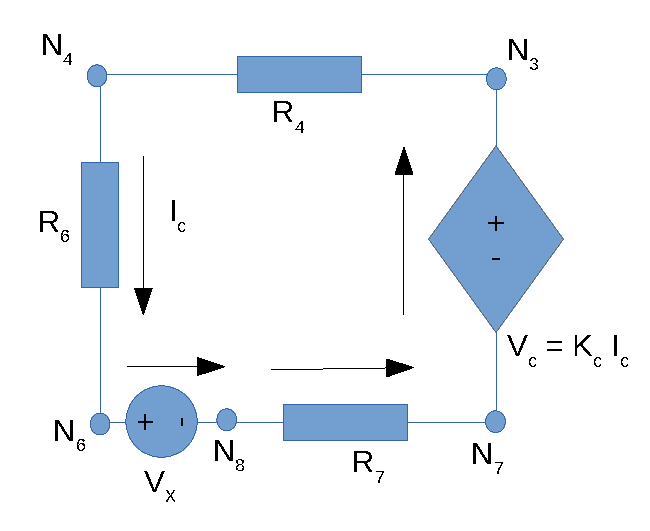
\includegraphics[width=0.6\linewidth]{malhaC.pdf}
\caption{C Mesh with an adicional voltage source} %mudar legendaaaaaaa
\label{fig:malhaC}
\end{figure}

In this simulation is important to explain the creation of an auxiliary voltage $V_b$ (with a voltage equal to $0V$) that was put between N6 and R7 as shown in Figure~\ref{fig:malhaC}. Consequently, this led to the appearance of a node that we designated by N8 that has the same voltage as N6.

This was necessary because of Ngspice software requirements.

By observing the Table~\ref{tab:op},Table~\ref{tab:nodal} and Table~\ref{tab:mesh} values it's possible to conclude that the simulated results are the same as the theoretical results.%são mesmo mesmo iguais?

\begin{table}[h]
  \centering
  \begin{tabular}{|l|r|}
    \hline    
    {\bf Name} & {\bf Value [A or V]} \\ \hline
    @cb[i] & 0.000000e+00\\ \hline
@ce[i] & 0.000000e+00\\ \hline
@q1[ib] & 7.022567e-05\\ \hline
@q1[ic] & 1.404513e-02\\ \hline
@q1[ie] & -1.41154e-02\\ \hline
@q1[is] & 5.765392e-12\\ \hline
@rc[i] & 1.411536e-02\\ \hline
@re[i] & 1.411536e-02\\ \hline
@rf[i] & 7.022567e-05\\ \hline
@rs[i] & 0.000000e+00\\ \hline
v(1) & 0.000000e+00\\ \hline
v(2) & 0.000000e+00\\ \hline
base & 2.254108e+00\\ \hline
coll & 5.765392e+00\\ \hline
emit & 1.411536e+00\\ \hline
vcc & 1.000000e+01\\ \hline

  \end{tabular}
  \caption{Operating point. A variable preceded by @ is of type {\em current}
    and expressed in Ampere; other variables are of type {\it voltage} and expressed in
    Volt.}
  \label{tab:op}
\end{table}

However, was also calculated the relative errors made in order to understand the accuracy of the results. 

Related to that calculations, it was noticed that in an experimental procedure, the calculation of relative errors is made by comparing experimental values and theorical values, meaning that the decimal places used in the theoretical value to be considered will be in accordance with the experimentally obtained places.


Considering that, in our case, the experimental values are obtained through NGSice, we must use theoretical values with the same number of decimal places returned by the simulation for calculating the errors, as it has a number of decimal places lower than that of the octave. By doing this calculating, all error values absolute and relative are equal to zero. 

Therefore, we can see that the order of magnitude of the errors will be residual.




